\section{Original Table}
\includegraphics[height=50mm]{text/pic_CEQ.pdf}


\section{Data from Rerun}
\begin{tabular}{||c||c|c||c|c||c|c||}
	\hline
	Grid Games&  \multicolumn{2}{|c||}{GG1} &
	 \multicolumn{2}{|c||}{GG2}  & \multicolumn{2}{|c||}{GG3}  \\ \hline
	Algorithm & Score & Games & Score & Games & Score & Games \\ \hline \hline
	%Q & Score & Games & Score & Games & Score & Games \\ \hline
	Friend-Q & $-10^{4},-10^{4}$ & 0 & $-10^{4},-10^{4}$ & 0 & $-10^{4},-10^{4}$ & 0 \\ \hline \hline
	uCE-Q & 100,100 & 2500 & 50,100 & 3333 & 117,117 & 3333 \\ \hline
	eCE-Q & 100,100 & 2500 & 100,50 & 3333 & 117,117 & 3333 \\ \hline
	rCE-Q & 100,100 & 2500 & 49,100 & 3333 & 100,125 & 3333 \\ \hline \hline
	lCE-Q & 100,100 & 2500 & 52, 100 & 3333 & $-10^{4},-10^{4}$ & 0 \\ \hline 
	
\end{tabular}

\section{Convergence}
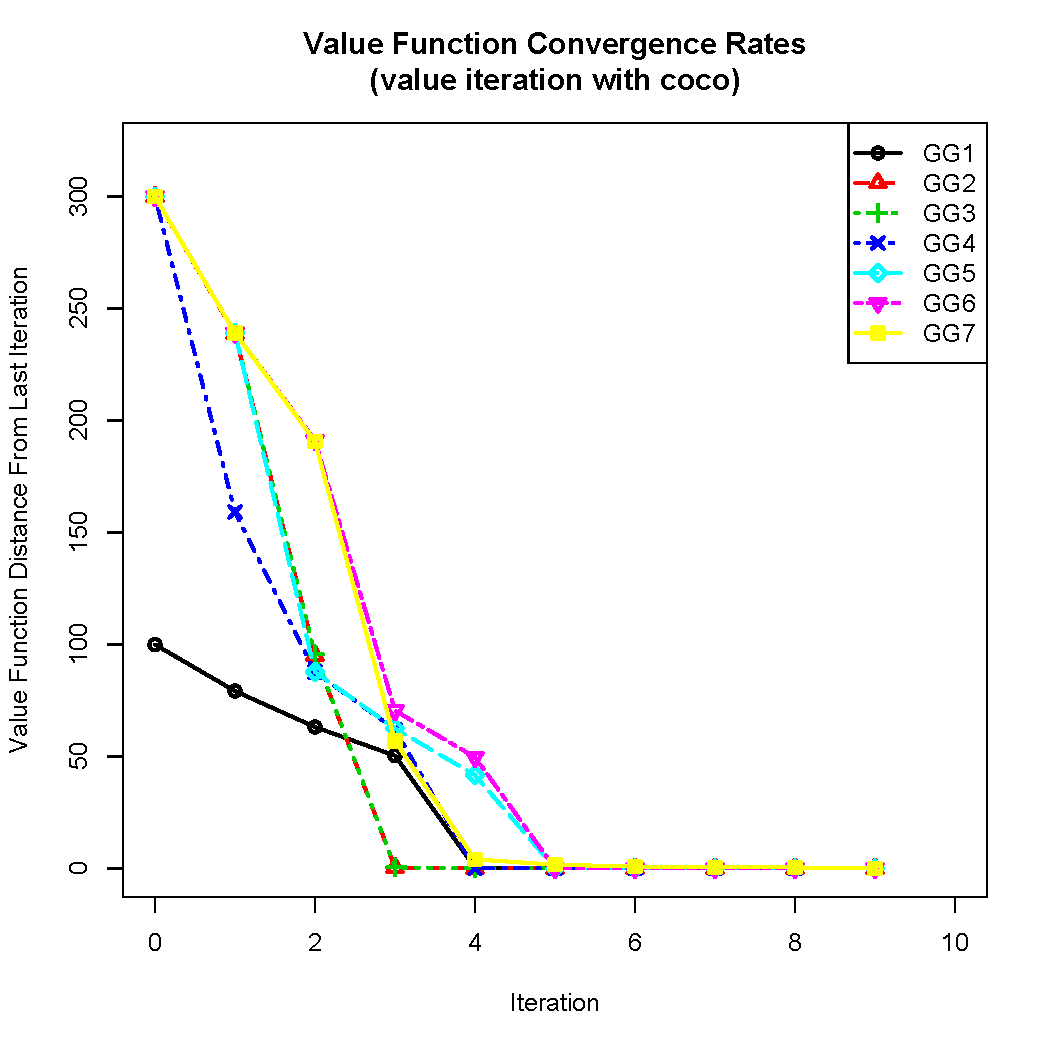
\includegraphics[height=90mm]{text/plot.pdf}

\section{Coco Agent Policies}
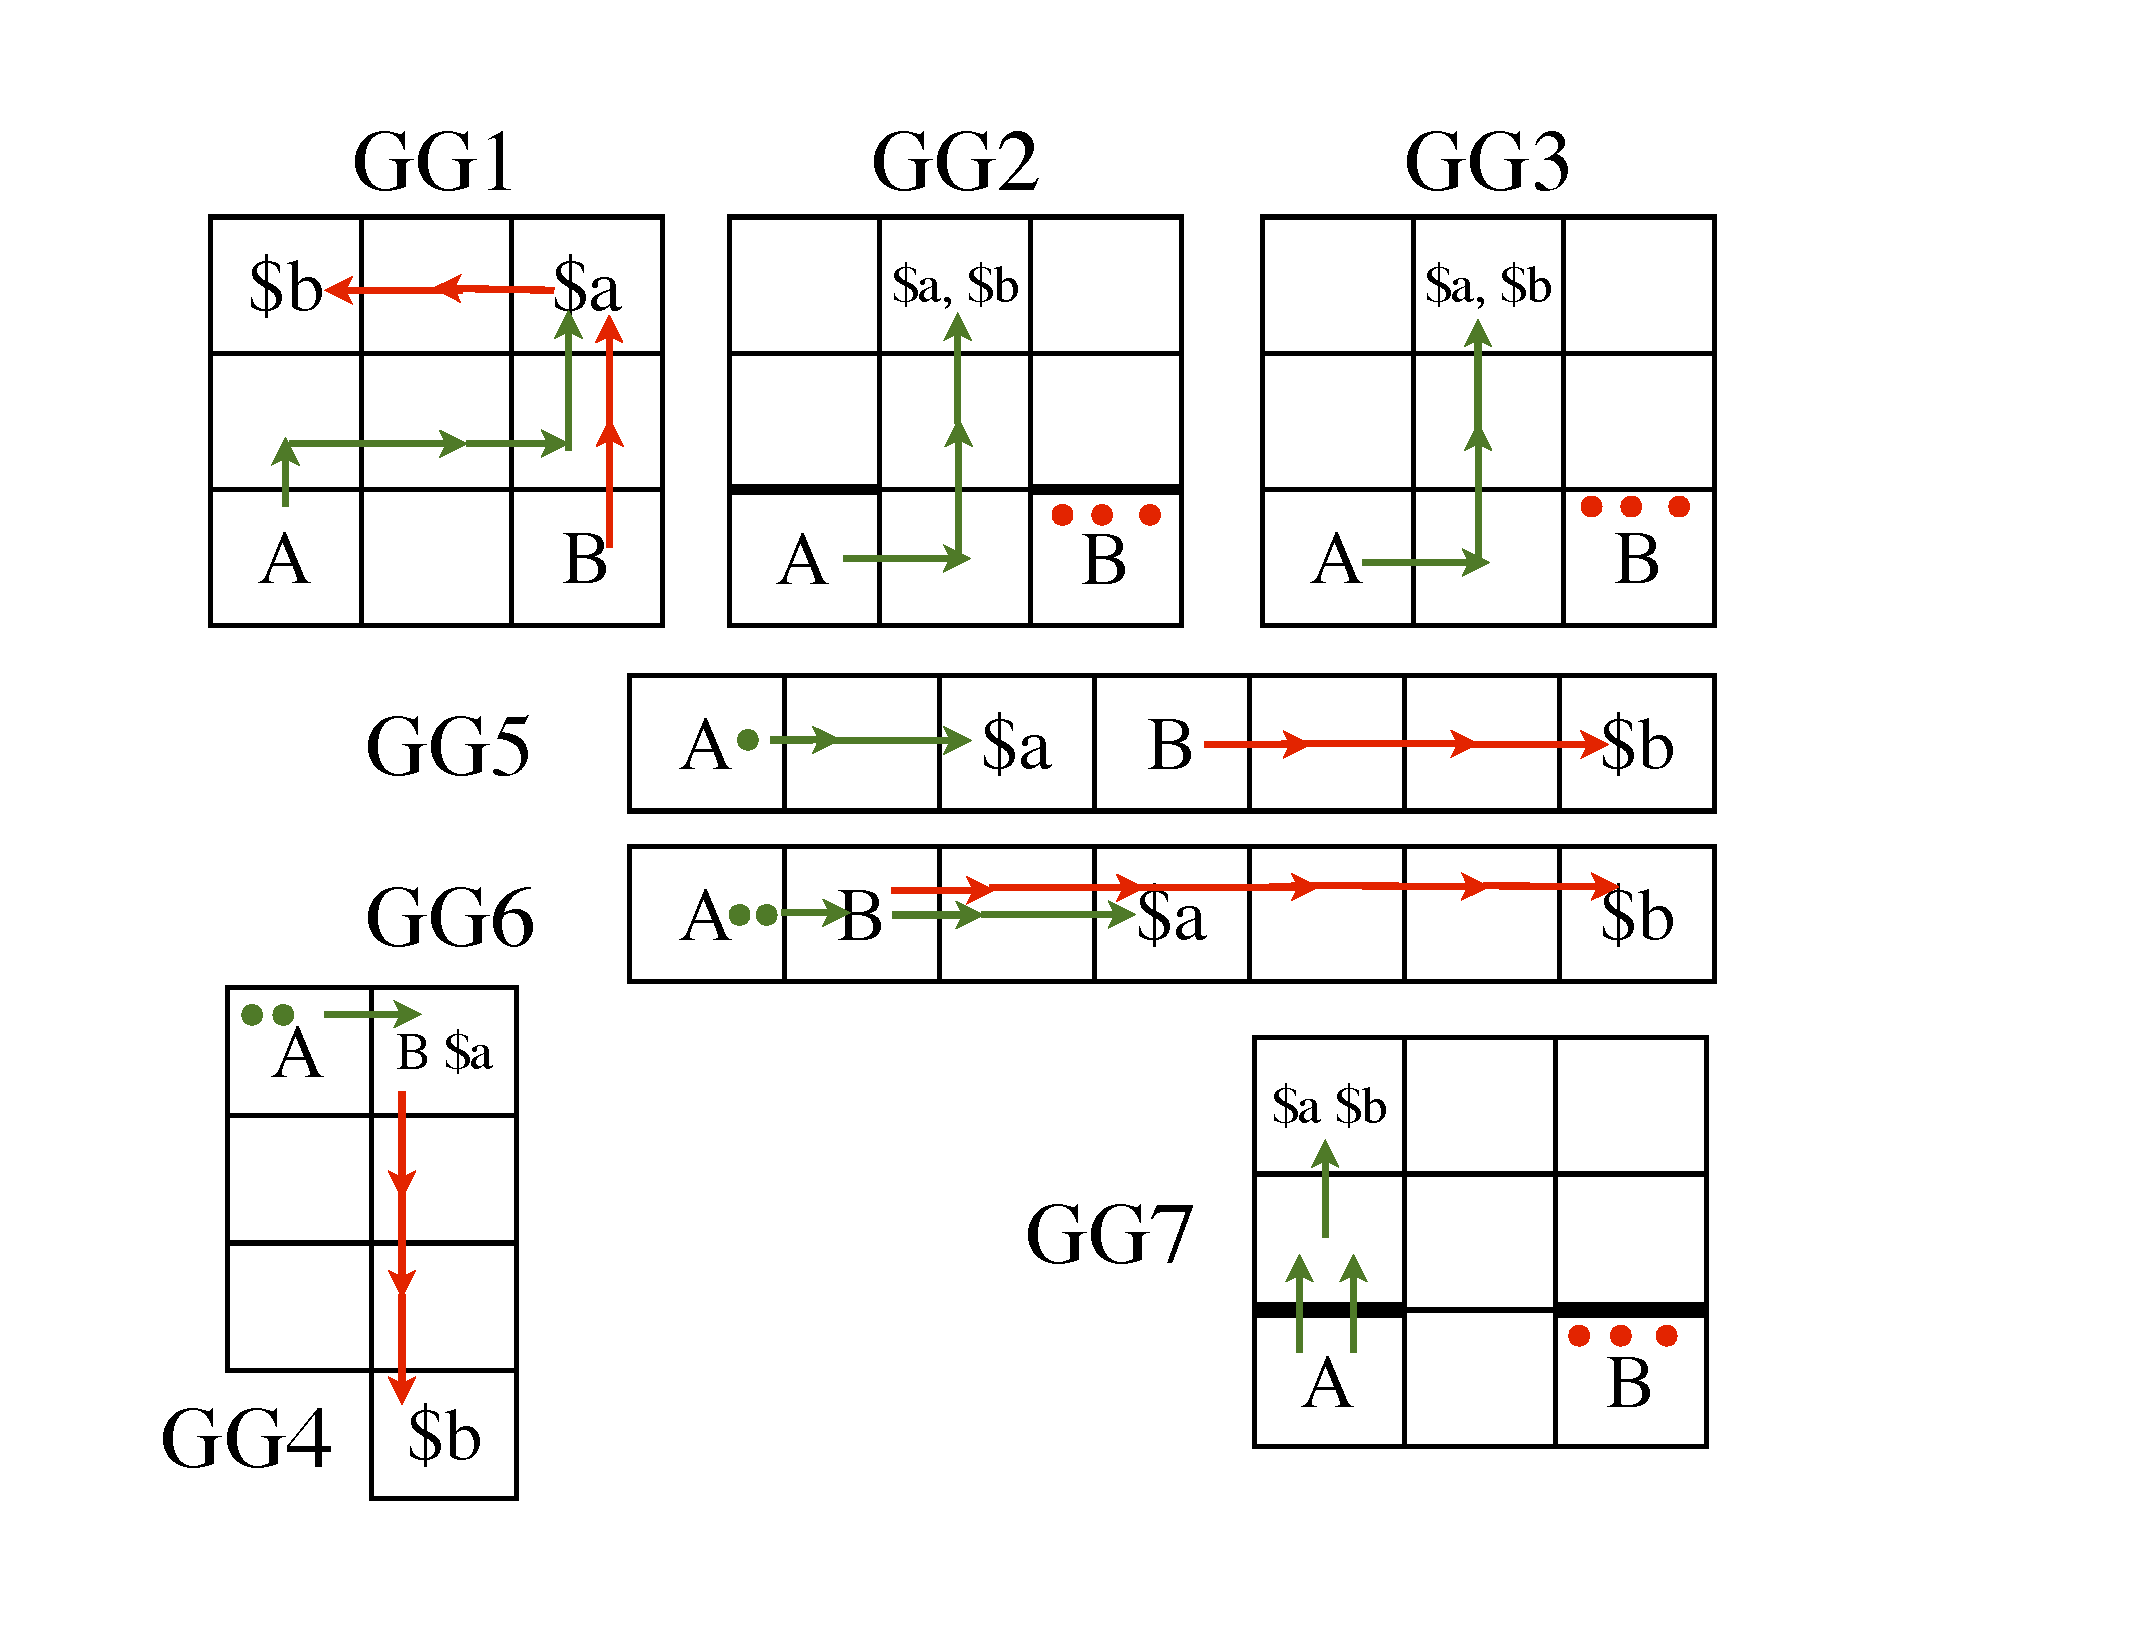
\includegraphics[height=90mm]{text/games.pdf}

%\section{VI for Nash and Coco Value agents}
%\begin{tabular}{||c||c|c||c|c||c|c||}
%	\hline
%	Solution Concept&  \multicolumn{3}{|c||}{Nash} &
%	 \multicolumn{3}{|c||}{Coco}  \\ \hline
%	Grid Game & Avg Reward & Deterministic?& Converge in: & Avg Reward & utility payments & Converge in: \\ \hline \hline
%	GG1 & Reward & yes & num Iter & Reward & utility trans. & num Iter\\ \hline
%	GG2 & Reward & yes & n num Iter & Reward & utility trans. & num Iter\\ \hline
%	GG3 & Reward & yes & n num Iter & Reward & utility trans. & num Iter\\ \hline
%	GG4 & 99.8, 0 & no & $\leq 10$ & Reward & utility trans. & num Iter\\ \hline
%	GG5 & 99.7, 99.6 & no & $\leq 10$ & Reward & utility trans. & num Iter\\ \hline
%	GG6 & 99.7, 99.5 & no & 35 & Reward & utility trans. & num Iter\\ \hline
%	GG7 & 99.8, 99.8 & yes & 3 & Reward & utility trans. & num Iter\\ \hline
%	GG8 & Reward & yes & n num Iter & Reward & utility trans. & num Iter\\ \hline
%	
%\end{tabular}
%
%\section{Games}
%\begin{tabular}{|c|c|}
%	\hline
%	 A &\$B, B   \\ \hline
%	 \hspace{6mm}  &\$A       \\ \hline
%	   &    \\ \hline
%    \multicolumn{1}{c|}{} & \$B \\ \hline
%\end{tabular}
%\begin{tabular}{|c|c|c|c|c|c|c|}
%	\hline
%	 A & B & \hspace{2mm} & \$A & \hspace{2mm} & \$B & \hspace{2mm} \\ \hline
%\end{tabular}
%\begin{tabular}{|c|c|c|c|c|c|c|}
%	\hline
%	 A & B & \hspace{2mm} & \$A & \hspace{2mm} & \hspace{2mm} & \$B\\ \hline
%\end{tabular}
%\begin{tabular}{|c|c|c|c|c|c|c|}
%	\hline
%	 A & B & \hspace{2mm} & \$A & \hspace{2mm} & \hspace{2mm} & \$B\\ \hline
%\end{tabular}
%\begin{tabular}{|c|c|c|c|}
%	\hline
%	 A & B & \$A & \$B\\ \hline
%\end{tabular}
%\begin{tabular}{|c|c|}
%	\hline
%	 A,\$B & B,\$A   \\ \hline
%	 \$B & \$A   \\ \hline
%\end{tabular}


